\subsubsection{\stid{1.11} Open MPI for Exascale (OMPI-X)}\label{subsubsect:openmpi}

%% {\itshape

%% 	\begin{enumerate}
%% 	\item Rename this file to your project WBS-projectname.tex, for example 2.3.3.01-XSDK4ECP.tex.
%% 	\item Complete this template for your project.  Limit your text to two pages, not counting citations.
%% 	\item Please avoid changing the content of main.tex.
%% 	\item Put any references in a .bib file with the same root name, for example 2.3.3.01-XSDK4ECP.bib.
%% 	\item Remember to include any image files you reference in your text.
%%     \item The files 2.3.3.01-XSDK4ECP.tex, 2.3.3.01-XSDK4ECP.bib and xSDK-diagram.jpeg are included as examples for your reference.  You can remove them from what you upload.
%% 	\end{enumerate}
%% }

\paragraph{Overview}
%% \textit{Provide an overview of your project.  You might find that the introductory text from your Fall 2017 Project Summary \url{https://confluence.exascaleproject.org/display/1ST/Fall+2017+ECP+ST+Project+Summaries} useful as a starting draft.}

The OMPI-X project ensures that the Message Passing Interface (MPI)
standard, and its specific implementation in Open MPI meet the needs
of the ECP community in terms of performance, scalability, and
capabilities or features. MPI is the predominant interface for
inter-process communication in high-end computing.  Nearly all of the
ECP application (AD) projects (93\%~\cite{Bernholdt:2018:SMU-tr})
and the majority of software technology (ST) projects
(57\%~\cite{Bernholdt:2018:SMU-tr}) rely on it.
%% Since its
%% inception, the MPI standard has evolved to address the changing needs
%% of massively parallel libraries and applications as well as the
%% systems on which they are run.
With the impending exascale era, the
pace of change and growing diversity of HPC architectures pose new
challenges that the MPI standard must address.  The OMPI-X project is
active in the MPI Forum standards organization, and works within it to
raise and resolve key issues facing ECP applications and libraries.

Open MPI is an open source, community-based implementation of the MPI
standard that is
%% freely available, and
used by a number of prominent
HPC vendors as the basis for their commercial MPI offerings.  The
OMPI-X team is comprised of active members of the Open MPI community,
with an extensive history of contributions to this community.
%% the development and
%% maintenance of the library.
The OMPI-X project focuses on prototyping
and demonstrating exascale-relevant proposals under consideration by
the MPI Forum, as well as improving the fundamental performance and
scalability of Open MPI, particularly for exascale-relevant platforms
and job sizes.  MPI users will be able to take advantage of these
enhancements simply by linking against recent builds of the Open MPI
library.

Without the OMPI-X project, there will be less competition and less
innovation in addressing the needs of ECP users in the critical area
of scalable, performant, and expressive exascale-quality inter-process
communication capabilities.

\paragraph{Key  Challenges}
%% \textit{Describe what is hard to do, why it is challenging.}
A number of aspects of ``exascale'' levels
of computing pose serious challenges to the ``tried and true'' message
passing model presented by MPI and its implementations, including Open
MPI.
%
Keeping pace with changes in HPC architecture is a major challenge.
The MPI ecosystem (the standard and its implementations) needs to
evolve to address challenges
%% on the programming side
driven by
architectural change, as well as taking advantage of new features and
capabilities.
%
As applications and libraries
%% they rely on
build up to exascale,
%% levels of computing and beyond,
the number of nodes, processes, and
threads required will rise significantly, whereas other key resources,
such as memory tend to go \emph{down} on a per-node, -process, or
-thread basis.  This emphasizes the importance of scalability in terms
of both performance and resource utilization.
%% to allow MPI to scale to
%% meet those needs.
%
Finally, we must work within the much larger and broader MPI
community to find approaches to address these challenges which do not
adversely impact the capabilities, performance, or scalability for
other users of MPI and Open MPI.

\paragraph{Solution Strategy}
%% \textit{Describe your basic strategy for addressing the challenges.}
The OMPI-X project is working across a number of fronts to address
these challenges.

\emph{Runtime Interoperability for MPI+X and Beyond} MPI is
increasingly being used concurrently with other runtime environments.
This includes both ``MPI+X'' approaches, where X
%% , in the ECP
%% environment, X
is most often a threading model, such as OpenMP, as
well as the use of multiple inter-process runtimes within a single
application.  Concerns include awareness of other runtimes,
cooperative resource management capabilities, and ensuring that all
concurrently active runtimes make progress.  We will develop APIs and
demonstrate capabilities for interoperability in both MPI+X and
multiple inter-process runtime situations.

\emph{Extending the MPI Standard to Better Support Exascale
Architectures} The MPI community is considering for standardization a
number of ideas that 
%% A number of ideas under consideration by the MPI
%% community for standardization
are particularly important to supporting
the architectural and system size characteristics anticipated for
exascale.  ``Finepoints'' and ``Endpoints''
%% are approaches to
deal
with the growing use of threading for node-level concurrency, in
combination with MPI.  ``Sessions'' increases the flexibility of MPI
semantics in a number of areas, which in turn can open opportunities
for enhanced scalability, as well as easier support for
multi-component applications such as coupled multi-physics
simulations.  We will develop prototype implementations and work with
ECP teams to evaluate the ability of these approaches to address ECP
requirements in order to facilitate the standardization process.

\emph{Open MPI Scalability and Performance} As we push the scale of
both hardware and applications, we stress MPI implementations and
expose areas that need to be improved in order to improve scalability.
OMPI-X is targeting memory usage within Open MPI, as well as remote
memory access (RMA), tag matching, and other areas, for improvements
in both scalability and performance.

\emph{Supporting More Dynamic Execution Environments} We are
developing and implementing strategies to help MPI applications
better deal with topological process layout preferences
%% as well as
%% responding to
and contention in the network.

\emph{Resilience in MPI and Open MPI} Concerns about system and
application resilience increase as either scales in size.
%% (number of
%% components or MPI ranks).
We will provide implementations of the
User-Level Fault Mitigation (ULFM) and ReInit proposals currently
under discussion within the MPI Forum, as well as demonstrations of
their use, in order to help drive standardization discussions, and to
help ECP team understand how they can take advantage of these
capabilities to improve the resilience of their libraries and
applications.

\emph{MPI Tools Interfaces}  Several interfaces within the
MPI standard are primarily used to support performance and
correctness tools.
%% of various kinds.
The MPI Forum is in the process
of making significant revisions and extensions to these interfaces.
We will track the discussions in the Forum and provide prototype
implementations within Open MPI to facilitate evaluation and provide
feedback.
%% on the standardization discussions.
We will work with the
ECP community, including tool developers, to make additional data
available through the MPI\_T interface.

\emph{Quality Assurance for Open MPI}  We are enhancing the
Open MPI testing infrastructure, adding tests to reflect ECP
requirements, and instantiating routine testing on systems of
importance to ECP.

\paragraph{Recent Progress}
%% \textit{Describe what you have done recently.  It would be good to
%% have some kind of figure or diagram in this section.}
The survey of MPI usage conducted last year continues to have impact
in the community.  In an article in The Next Platform in August
described our technical report \cite{Bernholdt:2018:SMU-tr} as a
``must read''.  Additionally, the MPI community, led in part by OMPI-X
team members, has launched a survey to obtain input from the broader
international MPI user community.

During the past year, we have ramped up our work in runtime
interoperability for ``MPI+X'' programming approachs.  We have
prototyped a capability to coordinate placement of ranks and threads
between MPI and OpenMP which cannot be achieved by ``standard''
methods.  This work has garnered significant interest in the community
and we forsee these activities expanding beyond our original
expectations.

%% We have delivered an implementation of the User-Level Fault Mitigation
%% (ULFM) resilience approach, which are under consideration by the MPI
%% Forum for inclusion in the standard.  ULFM provides the basic building
%% blocks for cheap, tailored recovery capabilities within applications
%% and libraries using MPI.  ULFM imposes no overhead on raw
%% communication performance on ECP-relevant hardware.  We are now
%% working with several application teams to demonstrate the capabilities
%% it provides.

%% \begin{wrapfigure}{r}{4in}
%% \begin{minipage}[c]{2in}
%% \vspace{0pt}
%% 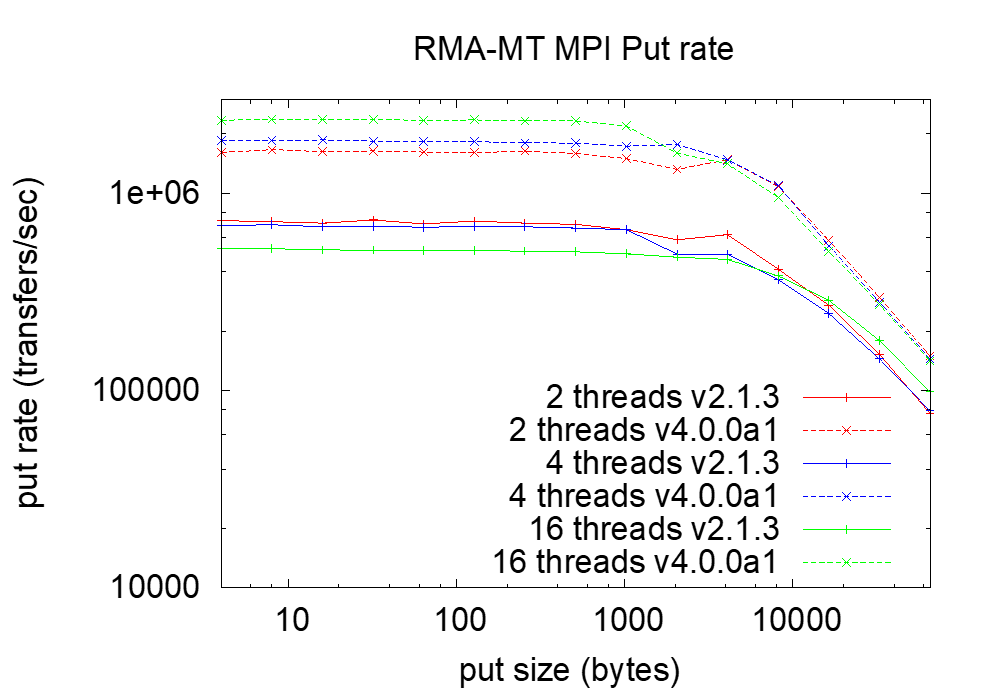
\includegraphics[width=\textwidth]{projects/2.3.1-PMR/2.3.1.11-OMPI-X/pritchard-rma-mt-put-rate.png}
%% \end{minipage}
%% \begin{minipage}[c]{2in}
%% \vspace{0pt}
%% 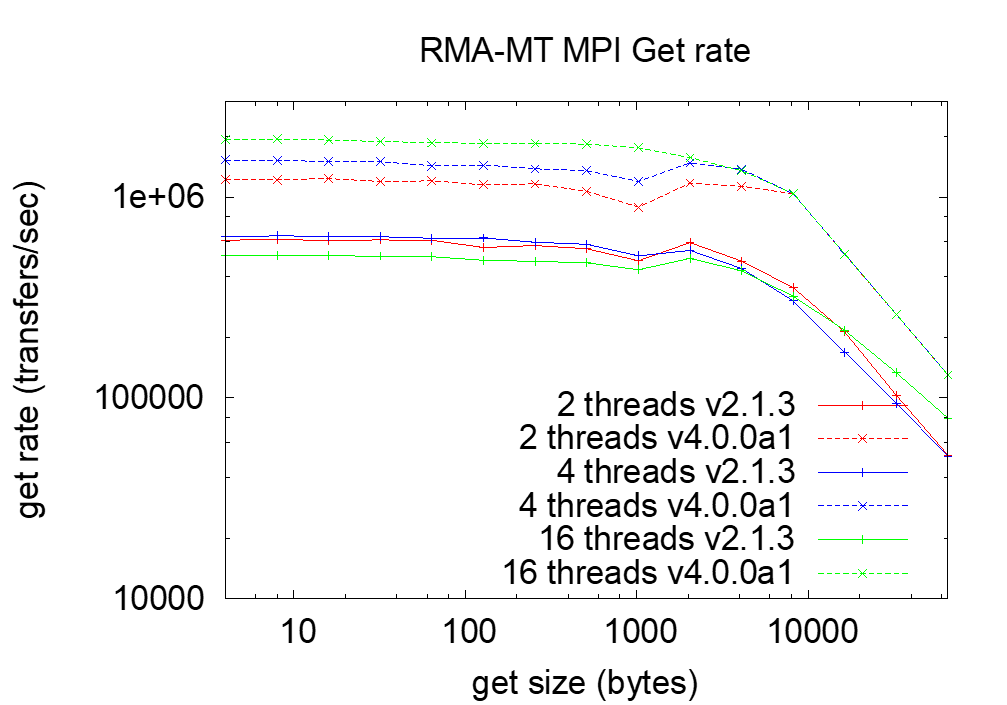
\includegraphics[width=\textwidth]{projects/2.3.1-PMR/2.3.1.11-OMPI-X/pritchard-rma-mt-get-rate.png}
%% \end{minipage}
%% \caption{Comparison of put (left) and get (right) RMA performance in a
%% multi-threaded context for Open MPI.  Recent OMPI-X contributions are
%% reflected in version 4.0.0a1 (top group of lines), in comparison with
%% v2.1.3.}
%% \label{fig:ompix-rma}
%% \end{wrapfigure}

The OMPI-X team has been active in the MPI Forum, driving
conversations about the Endpoints and Finepoints approaches to
supported threaded programming, and the Sessions concept, which will
improve the scalablity and flexibility of MPI.  Our prototype
Finepoints implementation shows improvements of 25\% in communicaton
time and 5\% in total runtime for an ECP mini-application.  New
aggregation techniques have been shown to provide 445\% increase in
communication bandwidth in certain cases.

The OMPI-X team is also active in other areas of the evolution of the
MPI standard. We have been driving development of the ``Sessions''
concept, will allow increased scalability in MPI applications and
implementations, as well as greater flexibility.
%
We are also tracking work on the PMPI tools interface replacement and
the enhancements to the MPI\_T tools interface.  We are working with
other members of the community to bring production-quality
implementations of these updated interfaces to Open MPI.

In the resilience area, we continued prior work on the User-Level
Fault Mitigation (ULFM) capability, fully integrating it into Open MPI
for the v4 release.  We also continue to pursue the ``Reinit'' fault
tolerance approach, completing the initial API design and plan for
implementation within Open MPI.

Behind the scenes of the Open MPI implementation, we are pursuing
efforts to improve performance and scalability, take full advantage of
the increasingly complex and sophisticated memory architectures that
are becoming available at the node level, and providing increased
topology and congestion awareness within the library.  We have made
improvements in RMA performance, which allows better scaling and
provides out-of-the-box performance in Open MPI which is comparable to
highly-tuned vendor implementations.  We have prototyped improved an
message matching implementation which improves matching performance by
up to 2x and saves significantly (1 GB) in memory, providing an
improvement in total runtime for on applicaton of 6\%.  We have also
worked to improve the MPI startup process by up to 5x in some
configurations.  And we have begun baselining memory utilization
in order to analyze and improve memory scalability.

%% We expect to be working on scalability and performance of Open MPI
%% throughout the project, but some early successes have been
%% demonstrated.  We have improved the RMA implementation so achieve
%% performance levels comparable to those obtained only by high tuned
%% implementations by vendors and significantly improved their
%% performance in multi-threaded contexts (Fig.~\ref{fig:ompix-rma}).  We
%% have also been able to improve message matching by up to 2$\times$
%% generally, and up to 45$\times$ on Intel Xeon Phi processors, and we
%% have made significant improvement to performance when MPI is used in a
%% multi-threaded environment.

%% %% Early work with the prototype implementation of Finepoints shows
%% %% improvements of 25\% in communication costs and 5\% in overall
%% %% execution time for one ECP mini-app.
%% %
%% Open MPI support for the MPI\_T interface has been extended~\cite{icl:957} to
%% provide a set of low-level counters to present a more detailed performance
%% characteristics map to tools and to users.
%
Finally, we continue to build out the MTT testing infrastructure and
continuous integration testing capabilities to provide better testing
capabilities for ECP-relevant platforms, including Summit at ORNL.

\paragraph{Next Steps}
%% \textit{Describe what you are working on next.}
We are making progress across multiple fronts, some of which has been
described above.  In FY19, we expect to continue our efforts on MPI+X
interoperability, pushing forward the Finepoints and Sessions
prototypes and standards proposals, as well as implementations of the
PMPI replacement and MPI\_T improvements.  We will also continue our
internal improvements in performance, scalability, and capabilities to
take maximum advantage of modern system capabilities. We are
tentatively planning to merge 2.3.1.15-Qthreads into OMPI-X in the
second phase of ECP ST activities due to the close technical and
personnel connections.
